\documentclass[smallextended]{svjour3}

\usepackage[boxruled]{algorithm2e}
\usepackage{amssymb}
\usepackage{amsmath}
\usepackage{booktabs} % Pandas dataframes
\usepackage{color}
\usepackage{enumerate} % Roman numerals
\usepackage{graphicx}
\usepackage{hyperref}
\usepackage{listings}
\usepackage{mathptmx}
\usepackage[square,sort,comma,numbers]{natbib}
\usepackage{subfig}
\usepackage{texments}
\usepackage{tikz}
    \usetikzlibrary{%
        arrows.meta,
        decorations.pathreplacing,
        decorations.text,
        patterns,
        shapes.arrows,
        shapes.geometric
    }


% Page setup and lengths
%\raggedbottom%

\newlength{\imgwidth}
\setlength{\imgwidth}{.96\textwidth}

\definecolor{deepblue}{rgb}{0,0,0.5}
\definecolor{deepred}{rgb}{0.6,0,0}
\definecolor{deepgreen}{rgb}{0,0.5,0}
\definecolor{cyan}{RGB}{0, 164, 216}
\definecolor{magenta}{RGB}{226, 62, 138}


% Algorithms and code
\newcommand{\balg}[1][htbp]{%
    \begin{algorithm}[#1]\DontPrintSemicolon
}
\newcommand{\ealg}{%
    \end{algorithm}
}

\lstset{
    backgroundcolor=,
	tabsize=4,
	rulecolor=,
	language=python,
        basicstyle=\scriptsize\ttfamily,
        aboveskip={1.5\baselineskip},
        breaklines=true,
        columns=fixed,
        identifierstyle=\ttfamily,
        keywordstyle=\color{deepblue},
        stringstyle=\color{deepgreen},
        commentstyle=\color{deepred},
        emphstyle=\color{deepred}
}

% TikZ styles, commands and settings
\pgfdeclarelayer{background}
\pgfsetlayers{background,main}

\tikzstyle{every picture} += [remember picture]
\tikzstyle{na} = [baseline=-.5ex]

\tikzset{%
    column/.pic={%
        code{%
            \draw[line width=1pt] (0, 0) rectangle (-2cm, 4cm);
            \foreach \val in {0, ..., #1}{%
                \draw[rotate=90] ([xshift=-\val*10pt] 4cm, 2cm) -- ++(0, -2cm);
            };
            \node at (-1cm, 1.25) {$\vdots$};
            \foreach \val in {1, 2}{%
                \draw (0, \val * 10pt) -- ++(-2cm, 0);
            };
        }
    }
}

\tikzset{%
    fullcolumn/.pic={%
        code{%
            \draw[line width=1pt] (0, 0) rectangle (-2cm, #1*10pt);
            \foreach \val in {0, ..., #1}{%
                \draw[rotate=90] ([xshift=-\val*10pt] #1*10pt, 2cm) -- ++(0, -2cm);
            };
        }
    }
}

\newcommand{\inputtikz}[3][.9\imgwidth]{%
    \begin{figure}[htbp]
        \centering
        \resizebox{#1}{!}{%
            \input{diag-#2.tex}
        }
        \caption{#3}\label{fig:#2}
    \end{figure}
}

\DeclareMathOperator*{\argmin}{arg\,min}
\renewcommand\theContinuedFloat{\alph{ContinuedFloat}}

% Document
\journalname{Data Mining and Knowledge Discovery}
\title{%
    Evolutionary Dataset Optimisation:
    learning algorithm quality through evolution
}
\author{%
    Henry Wilde \and
    Vincent Knight \and
    Jonathan Gillard
}
\institute{%
    School of Mathematics, Senghennydd Rd, Cardiff, WALES CF24 4AG\\
    \email{\{wildehd, knightva, gillardjw\}@cardiff.ac.uk}
}
\date{Received: date / Accepted: date}

\begin{document}

\maketitle%

\begin{abstract}
    When faced with a problem involving data, it is almost certainly the case
    that the data is fixed and in order to do something with that data, a
    researcher must select an algorithm that is appropriate for the problem
    domain whilst performing well on their data. The value prescribed to an
    algorithm is often found through a process of surveying the current
    literature to create a shortlist, then running various trials with the
    shortlisted algorithms. The winning algorithm is then chosen based on some
    common objective value. The issue with this process is that it does not
    necessarily allow (or require) the researcher to consider why certain
    algorithms perform better on particular datasets and not others, and which
    characteristics make data ``good'' for their chosen algorithm.

    This paper introduces a novel method for generating artificial data through
    genetic evolution, the purpose of which is to create populations of datasets
    for which a particular algorithm performs well. This is done by passing an
    algorithm's objective function to an evolutionary algorithm. Therein, each
    individual is a particular dataset defined by its dimensions, entries, and
    the approximate statistical shape of each of its attributes. In this way,
    detailed information about each individual is retained throughout the
    algorithm. Hence, they may be manipulated in a meaningful way during the
    run, and studied once the algorithm has terminated.

    Following this, a number of examples are given to show the performance of
    the method. These examples are created using a Python implementation of the
    process which is built to be highly customisable, interpretable and
    reproducible.
\end{abstract}


\section{Introduction}\label{section:introduction}

\inputtikz{flowchart}{%
    A general schematic for an evolutionary algorithm.
}

\begin{itemize}
    \item What is the motivation?\\
    Here, a diagram might be useful to highlight the flipped paradigm. Typically one would fix some benchmark examples and a metric, and then assess the algorithm based on this metric. This paradigm has a number of problems:\\
    1. How were the benchmark examples selected? In some disciplines/domains there are well established benchmarks, in others less so. Sometimes a `new' data set is simulated to assess the performance of an algorithm. How and why is this simulation created?\\
    2. In disciplines where there are established benchmarks, there still may be problems e.g. (i) Work by Hyndman, who considered benchmark data sets used in time series analysis competitions, showed that the data sets were biased towards particular attributed; (ii) the amount of learning one can gain as to the attributes of data which lead to good (or bad) performance of an algorithm are constrained to the finite set of attributes present in the benchmark data chosen in the first place.
    \item What is the problem?
    \item What is the solution?
\end{itemize}

%-----------------------------
\subsection{Literature review}

\begin{itemize}
    \item How is artificial data made?
    \item Why hasn't this been done before?
    \item Genetic algorithms used to train algorithms for data
    \item Diagram showing that this is the ``reverse'' problem
\end{itemize}

\section{The evolutionary algorithm}\label{section:algorithm}

\subsection{Structure}

In this section, the details of an algorithm that generates data for which a
given function or, equivalently, an algorithm which is well suited, is
described. This algorithm is to be referred to as ``Evolutionary Dataset
Optimisation'' (EDO).

The EDO method is built as an evolutionary algorithm which follows a traditional
(generic) schema with some additional features that keep the objective of
artificial data generation in mind. With that, there are a number of parameters
that are passed to EDO;\ the typical parameters of an evolutionary algorithm
are a fitness function, \(f\), which maps from an individual to a real number,
as well as a population size, \(N\), a maximum number of iterations, \(M\), a
selection parameter, \(b\), and a  mutation probability, \(p_m\). In addition to
these, EDO takes the following parameters:

\begin{itemize}
    \item Limits on the number of rows an individual dataset can have:
        \[
            R \in \left\{%
                (r_{\min}, r_{\max}) \in \mathbb{N}^2~|~r_{\min} \leq r_{\max}
            \right\}
        \]
    \item Limits on the number of columns a dataset can have:
        \[
            C := \left(C_1, \ldots, C_{|\mathcal{P}|}\right)
            ~\text{where}~
            C_j \in \left\{ (c_{\min}, c_{\max}) \in {%
                \left(\mathbb{N}\cup\{\infty\}\right)
            }^2~|~c_{\min} \leq c_{\max}\right\}
        \]
        for each \(j = 1, \ldots, |\mathcal{P}|\). That is, \(C\) defines the
        minimum and maximum number of columns a dataset may have from each
        distribution in \(\mathcal{P}\).
    \item A set of probability distribution families, \(\mathcal{P}\). Each
        family in this set has some parameter limits which form a part of the
        overall search space. For instance, the family of normal distributions,
        denoted by \(N(\mu, \sigma^2)\), would have limits on values for the
        mean, \(\mu\), and the standard deviation, \(\sigma\).
    \item A probability vector to sample distributions from \(\mathcal{P}\),
        \(w = \left(w_1, \ldots, w_{|\mathcal{P}|}\right)\).
    \item A second selection parameter, \(l \in [0, 1]\), to allow for a
        small proportion of ``lucky'' individuals to be carried forward.
    \item A shrink factor, \(s \in [0, 1]\), defining the relative size of a
        component of the search space to be retained after adjustment.
\end{itemize}

The concepts discussed in this section form the mechanisms of the evolutionary
dataset optimisation algorithm. To use the algorithm practically, these
components have been implemented in Python as a library built on the scientific
Python stack~\cite{pandas,numpy}. The library is fully tested and documented (at
\url{https://edo.readthedocs.io}) and is freely available online under the MIT
license~\cite{edo-project}. The EDO implementation was developed to be
consistent with the best practices of open source software development.
% TODO Citation(s) needed.

\balg%
\KwData{%
    \begin{tabular}{l}
    Fitness function, \(f: X \to \mathbb{R}\);
    population size, \(N\);
    row limits, \(R = [r_l, r_u]\);
    column limits, \(C = [c_l, c_u]\);\\

    Column distributions, \(P\);
    relative weights for \(P\), \(w \in {[0, 1]}^{|P|}\) s.t.\ \(\sum w = 1\);
    maximum iterations, \(M\);\\

    Best proportion, \(\delta\);
    lucky proportion, \(\epsilon\);
    mutation probability, \(\mu\);
    compaction ratio, \(s\).
    \end{tabular}
}
\KwResult{A full history of the populations and their fitnesses.}\;

\textcolor{blue}{initialisation}\;
\(population \longleftarrow CreateInitialPopulation(N,R,C,P,w)\)\;
\(populationFitness \longleftarrow GetPopulationFitness(population,f)\)\;
\(%
    populationHistory \longleftarrow%
    \left\{(population, populationFitness)\right\}
\)\;
\(i \longleftarrow 0\)\;\;

\textcolor{blue}{begin iterative step}\;
\While{\(iteration < M\) and not \textbf{STOP}}{%
    \textcolor{blue}{select parent individuals}\;
    \(%
        parents \longleftarrow%
        Selection(population,populationFitness,\delta,\epsilon)
    \)\;

    \textcolor{blue}{create new population}\;
    \(population \longleftarrow CreateNewPopulation(parents,N,R,C,P,w,\mu)\)\;

    \textcolor{blue}{update fitness and history}\;
    \(populationFitness \longleftarrow GetPopulationFitness(population,f)\)\;
    \(%
        populationHistory \longleftarrow%
        populationHistory \cup \left\{(population,populationFitness)\right\}
    \)\;

    \textcolor{blue}{adjust parameters}\;
    \(i \longleftarrow i + 1\)\;
    \(P \longleftarrow ReduceMutationSpace(parents,P,i,M,s)\)\;
    \(\mu, \textbf{STOP} \longleftarrow UpdateParameters\)\;
}
\caption{The evolutionary dataset optimisation algorithm}
\ealg%
\label{alg:edo}
\balg%
\KwData{\(parents,N,R,C,P,w,\mu\)}
\KwResult{A new population of size \(N\), \(newPopulation\)}\;

\(newPopulation \longleftarrow parents\)\;
\While{\(|newPopulation| < N\)}{%
    Sample two parents, \(parentOne, parentTwo\), from \(parents\)\;
    \(offspring \longleftarrow Crossover(parentOne,parentTwo,C,P,)\)\;
    \(mutant \longleftarrow Mutation(offspring,\mu,R,C,P,w)\)\;
    \(newPopulation \longleftarrow newPopulation \cup \{mutant\}\)\;
}
\caption{\(CreateNewPopulation\)}
\ealg%


The statement of the EDO algorithm is presented here to lay out its general
structure from a high level perspective. Lower level discussion is provided
below where additional algorithms for the individual creation, evolutionary
operator and shrinkage processes are given along with diagrams (where
appropriate).

Note that there are no defined processes for how to stop the algorithm or adjust
the mutation probability, \(p_m\). This is down to their relevance to a
particular use case. Some examples include:

\begin{itemize}
    \item Stopping when no improvement in the best fitness is found within some
        \(K\) consecutive iterations~\cite{Leung2001}.
    \item Utilising global behaviours in fitness to indicate a stopping
        point~\cite{Marti2016}.
    \item Regular decreasing in mutation probability across the available
        attributes~\cite{Kuehn2013}.
\end{itemize}

\subsection{Individuals}

Evolutionary algorithms operate on succeeding populations of individuals often
coined as ``generations''. In a genetic algorithm, an individual would be
encoded as a bit string of a fixed length and treated as a chromosome-like
object to be manipulated. In EDO, as it is an evolutionary algorithm and the
objective is to generate datasets, there is no encoding process. Instead, the
datasets are manipulated directly so that the biological operators can be
designed and be interpreted in a more meaningful way.

\inputtikz{individual}{%
    An example of how an individual is first created.
}

In a sense, a dataset is treated similarly to a bit string in a genetic
algorithm as the primary components of the dataset are considered to be its
columns. As is seen in Figure~\ref{figure:individual}, an individual's creation
is defined by the generation of its columns. A set of instructions on how to
sample new values for that column are recorded in the form of a probability
distribution. These distributions are sampled from \(\mathcal{P}\).

A caveat to this: one should not assume that the columns are a reliable
representative of the distribution associated with them, or vice versa. This is
particularly true of ``shorter'' datasets with a small number of rows, whereas
confidence in the pair could be given more liberally for ``longer'' datasets
with a larger number of rows. In any case, appropriate methods should be
employed to understand the structure and characteristics of the data produced
before formal conclusions are made.

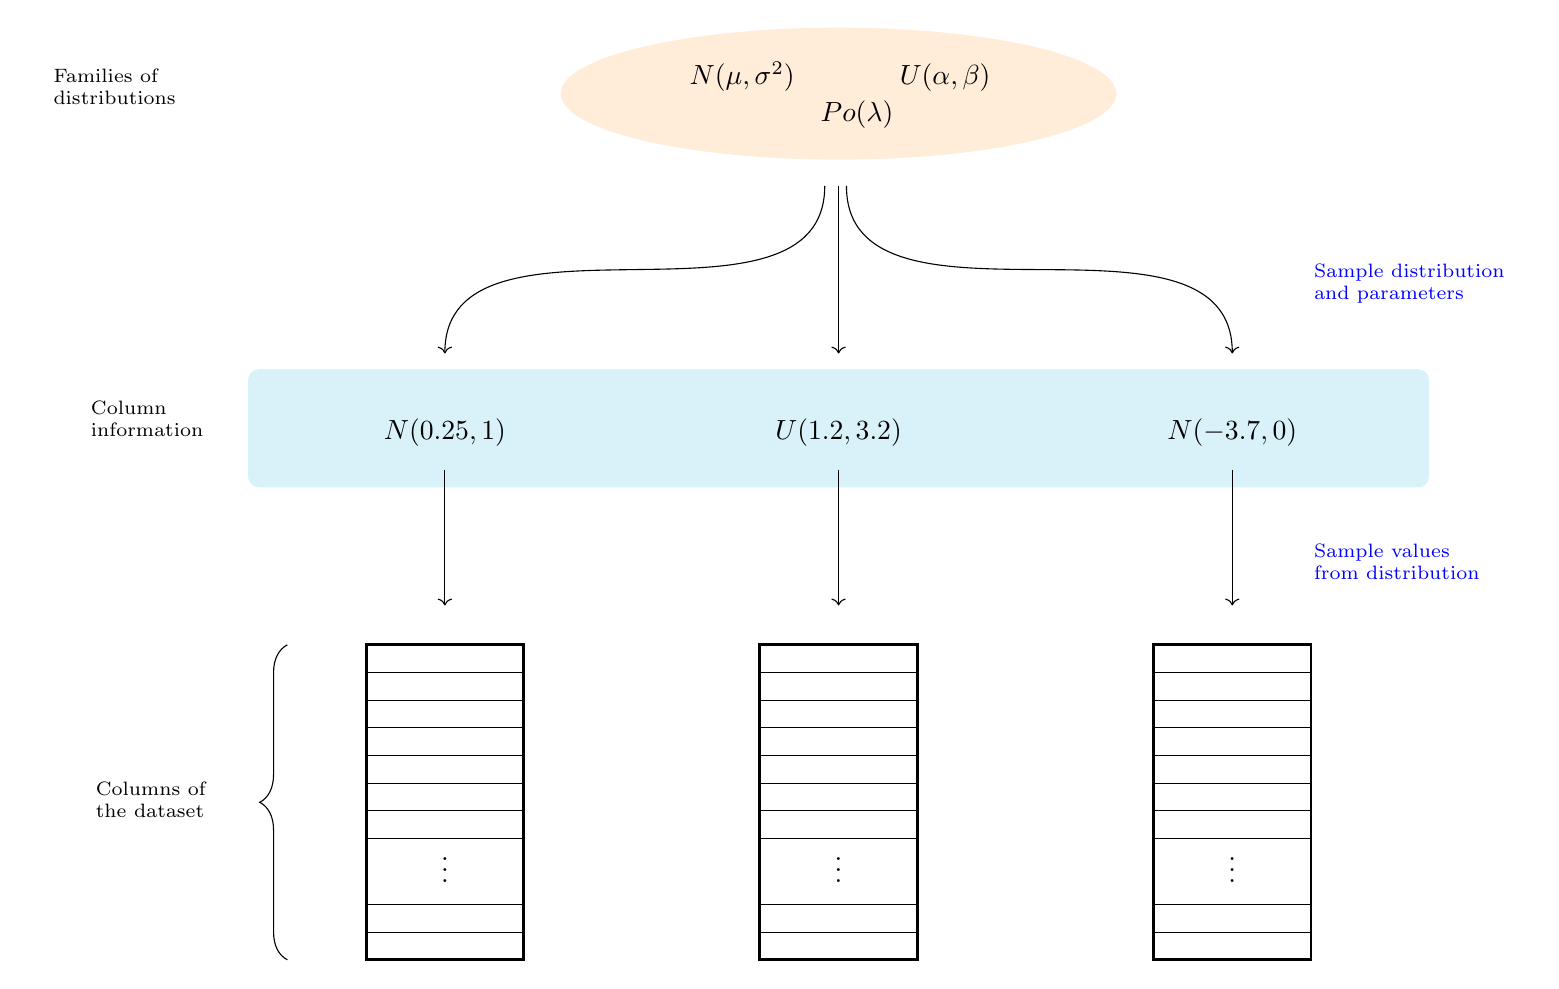
\begin{tikzpicture}

    \path (-4, -10) pic {column=7}
          (1, -10) pic {column=7}
          (6, -10) pic {column=7};

    \node[ellipse, fill=orange!15] (dists) at (0, 1) {%
        \begin{tabular}{c}
            \tikz[baseline, inner sep=0] \node[anchor=base] (normal) {$N(\mu,
            \sigma^2)$}; \quad \quad \tikz[baseline, inner sep=0]
            \node[anchor=base] (uniform) {$U(\alpha, \beta)$}; \\
            {} \quad $Po(\lambda)$
        \end{tabular}
    } node[yshift=30pt, left=230pt] {%
        \scriptsize
        \begin{tabular}{l}
            Families of\\
            distributions
        \end{tabular}
    };

    \fill[cyan!15, rounded corners] node[yshift=-90pt,left=220pt] 
        {%
            \color{black}\scriptsize
            \begin{tabular}{l}
                Column\\
                information
            \end{tabular}
        }
        (-7.5,-4) rectangle (7.5,-2.5);
    
    \node (norm1) at (-5, -3.3) {$N(0.25, 1)$};
    \node (norm2) at (5, -3.3) {$N(-3.7, 0)$};
    \node (uniform1) at (0, -3.3) {$U(1.2, 3.2)$};

    \draw[->] ([xshift=-5pt] normal.south) to [out=270, in=90]
        ([yshift=1cm] norm1);
    \draw[->] ([yshift=-5pt] norm1.south) -- (-5, -5.5);

    \draw[->] ([xshift=0.1cm] normal.south) to [out=270, in=90]
        ([yshift=1cm] norm2) node[right=20pt, yshift=25pt] {%
            \color{blue}\scriptsize
            \begin{tabular}{l}
                Sample distribution\\
                and parameters
            \end{tabular}
        };
    \draw[->] ([yshift=-5pt] norm2.south) to (5, -5.5)
        node[right=20pt, yshift=15pt] {%
            \color{blue}\scriptsize
            \begin{tabular}{l}
                Sample values\\
                from distribution
            \end{tabular}
        };

    \draw[->] (uniform) to [out=270, in=90] ([yshift=1cm] uniform1);
    \draw[->] ([yshift=-5pt] uniform1.south) -- (0, -5.5);

    \draw[decorate, decoration={brace, amplitude=10pt}] (-7, -10) -- (-7, -6)
    node[midway, left=20pt] {%
        \scriptsize
        \begin{tabular}{l}
            Columns of\\
            the dataset
        \end{tabular}
    };

\end{tikzpicture}


\subsection{Selection}

The selection operator describes the process by which individuals are chosen
from the current population to generate the next. Almost always, the likelihood
of an individual being selected is determined by their fitness. This is because
the purpose of selection is to preserve favourable qualities and encourage some
homogeneity within future generations~\cite{Back1994}.

\inputtikz[.8\textwidth]{selection}{%
    The selection process with the inclusion of some lucky individuals.
}
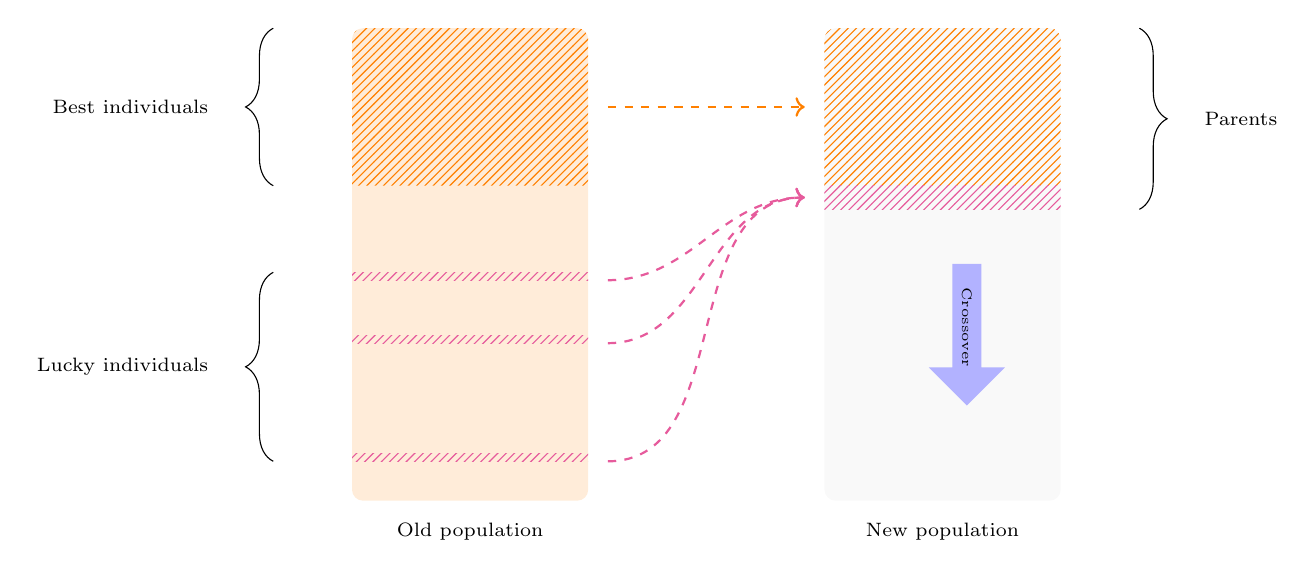
\begin{tikzpicture}

    \fill[orange!15, rounded corners] (0, 0) rectangle (3, -6)
        node[below=90pt, midway] {\color{black} \scriptsize Old population};
    \fill[rounded corners, gray!5] (6, 0) rectangle (9, -6)
        node[below=90pt, midway] {\color{black} \scriptsize New population};

    \fill[pattern=north east lines, pattern color=orange]
        (0, -2) --
        ++(3, 0) {[rounded corners] --
        ++(0, 2) --
        ++(-3, 0)} --
        cycle
        {};
   
    \draw[->, dashed, orange, thick] (3.25, -1) to (5.75, -1);

    \fill[pattern=north east lines, pattern color=orange]
        (6, -2) --
        ++(3, 0) {[rounded corners] --
        ++(0, 2) --
        ++(-3, 0)} --
        cycle
        {};

    \foreach \val in {-5.5, -4, -3.2} {%
        \fill[pattern=north east lines, pattern color=magenta!85]
            (0, \val) rectangle (3, \val+0.1);
        \draw[->, dashed, magenta!85, thick]
            (3.25, \val) to [out=0, in=180] (5.75, -2.15);
    };

    \fill[pattern=north east lines, pattern color=magenta!85]
        (6, -2.3) rectangle (9, -2);

    \draw[decorate, decoration={brace, amplitude=10pt}] (-1, -2) -- (-1, 0)
        node[midway, left=20pt] {\scriptsize Best individuals};
    \draw[decorate, decoration={brace, amplitude=10pt}] (-1, -5.5) -- (-1, -3.1)
        node[midway, left=20pt] {\scriptsize Lucky individuals};
    \draw[decorate, decoration={brace, amplitude=10pt}] (10, 0) -- (10, -2.3)
        node[midway, right=20pt] {\scriptsize Parents};

    \node[%
        fill=blue!30, single arrow, minimum height=18mm, minimum width=4mm,
        single arrow head extend=3mm, anchor=north, rotate=-90]
        at (8, -3.8) {\tiny Crossover};

\end{tikzpicture}


In EDO, a modified truncation selection method is used, as can be seen in
Figure~\ref{figure:selection}. Truncation selection takes a fixed number, \(n_b
= \lceil bN\rceil\), of the fittest individuals in a population and makes them
the ``parents'' of the next. The modification is an optional stage after the
best individuals have been chosen: by passing some small \(l\) to the
evolutionary algorithm, a number of the remaining individuals can be selected at
random to be carried forward. This number is given by \(n_l = \lceil lN
\rceil\). It should be noted that even with this modification, no individual may
be selected more than once in a single iteration but could potentially be
present throughout the run of the algorithm.

It has been shown that, despite its efficiency as a selection operator,
truncation selection can lead to premature convergence at local
optima~\cite{Jebari2013, Tatsuya2002}. Hence, allowing for the inclusion of a
small number of randomly selected individuals may encourage diversity and
exploration throughout the run of the algorithm.

\subsection{Crossover}

Crossover is the operation of combining two individuals in order to create at
least one offspring. In EDO, a method known as uniform crossover is
used~\cite{Semenkin2012}. Under this method, a new individual is created by
uniformly sampling each of its
components from a set of two ``parent'' individuals. As can be seen in
Figure~\ref{figure:crossover}, this method has been adapted for the dataset
representation, i.e.\ two parent datasets have their dimensions and then columns
sampled uniformly and without replacement to give a new individual.

\inputtikz{crossover}{The crossover process.}
\subsection{Crossover}

Crossover is the operation of combining two individuals in order to create at
least one offspring. In EDO, a method known as uniform crossover is
used~\cite{Semenkin2012}. Under this method, a new individual is created by
uniformly sampling each of its
components from a set of two ``parent'' individuals. As can be seen in
Figure~\ref{figure:crossover}, this method has been adapted for the dataset
representation, i.e.\ two parent datasets have their dimensions and then columns
sampled uniformly and without replacement to give a new individual.

\inputtikz{crossover}{The crossover process.}
\subsection{Crossover}

Crossover is the operation of combining two individuals in order to create at
least one offspring. In EDO, a method known as uniform crossover is
used~\cite{Semenkin2012}. Under this method, a new individual is created by
uniformly sampling each of its
components from a set of two ``parent'' individuals. As can be seen in
Figure~\ref{figure:crossover}, this method has been adapted for the dataset
representation, i.e.\ two parent datasets have their dimensions and then columns
sampled uniformly and without replacement to give a new individual.

\inputtikz{crossover}{The crossover process.}
\input{tex/algorithms/crossover.tex}





\subsection{Mutation}

Mutation is used in evolutionary algorithms to encourage a broader exploration
of the search space at each generation. Under this framework, the mutation
process acts on each characteristic of an individual: the dimensions, the column
metadata and the entries themselves. This process is described in
Figure~\ref{figure:mutation}, and is such that all aspects of the search space
are susceptible to mutation.

\inputtikz{mutation}{The mutation process.}

Each of the potential mutations occur with the same probability, \(p_m\), but
the way in which columns are maintained assure that (assuming appropriate
choices for \(f\) and \(\mathcal{P}\)) many mutations in the metadata and the
dataset itself will only result in some incremental change in the individual's
genetics and fitness overall \-- at least relatively so to, say, a completely
new individual.

\balg%
\KwData{An individual, \(p_m\), \(R\), \(C\), \(\mathcal{P}\), \(w\)}
\KwResult{A mutated individual}

\Begin{%
    sample a random number \(r \in [0, 1]\)\;
    \If{\(r < p_m\) and adding a row would not violate \(R\)}{%
        sample a value from each distribution in the metadata\;
        append these values as a row to the end of the dataset\;
    }
    sample a new \(r \in [0, 1]\)\;
    \If{\(r < p_m\) and removing a row would not violate \(R\)}{%
        remove a row at random from the dataset
    }
    sample a new \(r \in [0, 1]\)\;
    \If{\(r < p_m\) and adding a new column would not violate \(C\)}{%
        create a new column using \(\mathcal{P}\) and \(w\)\;
        append this column to the end of the dataset
    }
    sample a new \(r \in [0, 1]\)\;
    \If{\(r < p_m\) and removing a column would not violate \(C\)}{%
        remove a column (and its associated metadata) at random from the dataset
    }
    \For{each distribution in the metadata}{%
        \For{each parameter of the distribution}{%
            sample a random number \(r \in [0, 1]\)\;
            \If{\(r < p_m\)}{%
                update the parameter value by sampling a new value from the
                associated distribution parameter limits
            }
        }
    }
    \For{each value in the dataset}{%
        sample a random number \(r \in [0, 1]\)\;
        \If{\(r < p_m\)}{%
            update the value by sampling a new value from the associated
            distribution in the metadata
        }
    }
}
\caption{The mutation process}
\ealg%


\subsection{Shrinking}

The potential benefits of adapting the search space of an EA has been
well-discussed in the domain of complex optimisation problems. During the
development of EDO, two methods were considered to do this. Each of these
methods relied on a law relating a successive generation's search space with its
predecessor. It should be noted that in both cases the methods were adapted to
conform with the choice to represent individuals as they are rather than as bit
strings.

The first was developed to be a two-part process based on a linear law with two
parameters: a shrink factor, \(s \in (0, 1)\), and the maximum number of
iterations \(M \in \mathbb{N}\)~\cite{Amirjanov2017}. The adapted method would
be as follows. For all iterations, \(t \geq sM\), no shrinking would take place.
However, for all previous iterations, the suggested method would take the
parents found during selection and act on each component of the search space.
That is, for each iteration, \(t < sM\), every component would have its lower
and upper limits, denoted by \(l_t\) and \(u_t\) respectively, adjusted so that
they are centred about the mean parent value, \(\mu\), and be such that:
\[
    u_{t+1} - l_{t+1} = (u_t - l_t) \left(1 - \frac{t}{sM}\right)
\]

More specifically, the adjusted limits would be calculated as follows:
\begin{align*}
    l_{t+1} = \max \left\{%
        l_t, \ \mu - \frac{1}{2} (u_t - l_t) \left(1 - \frac{t}{sM}\right)
    \right\}\\
    u_{t+1} = \min \left\{%
        u_t, \ \mu + \frac{1}{2} (u_t - l_t) \left(1 - \frac{t}{sM}\right)
    \right\}
\end{align*}

The second method was for use in a genetic algorithm which mapped weighted bit
strings to some pre-defined interval with lower and upper
bounds~\cite{Amirjanov2016}. The proposed method would rely on a power law with
a single parameter: some shrink factor, \(s \in [0, 1]\). Again, at each
iteration, the parents would be taken and every component's limits would be
adjusted so that they were centred about the mean parent value, \(\mu\), such
that:
\[
    u_{t+1} - l_{t+1} = (u_t - l_t) s^t
\]

The process by which the values of \(l_{t+1}\) and \(u_{t+1}\) would be found
are equivalent to the above but with a different shift term:
\begin{align}
    \label{eq:shrinking_lower}
    l_{t+1}&= \max \left\{l_t, \ \mu - \frac{1}{2} (u_t - l_t) s^t\right\}\\
    \label{eq:shrinking_upper}
    u_{t+1}&= \max \left\{u_t, \ \mu + \frac{1}{2} (u_t - l_t) s^t\right\}
\end{align}

From these brief definitions alone, these methods appear to be largely
indistinguishable. However, following a wider discussion around how EDO would
work for the general user, it was decided that the first method be rejected in
favour of the second. It was found that the second method having fewer
parameters was a particularly redeeming feature; this removed any hidden or
otherwise unwanted interactions between a parameter dedicated to the shrink
process, \(s\), and the maximum number of iterations, \(M\), which is often used
as a fallback stopping criterion in complex problem domains.

\balg%
\KwData{parents, current iteration, \(\mathcal{P}, M, s\)}
\KwResult{A new mutation space focussed around the parents}

\Begin{%
    calculate the shrink coefficient\;

    \For{distribution in \(\mathcal{P}\)}{%
        \For{each parameter of the distribution}{%
            get current values for parameter in parent columns\;
            find the mean value\;
            calculate the shift term using the values and shrink coefficient\;
            find the new lower and upper bounds around the mean\;
            set the parameter limits\;
        }
    }
}
\caption{Shrinking the mutation space}
\ealg%



\section{Examples}\label{section:examples}

\subsection{\(k\)-means clustering}

The following examples act as a form of validation for EDO, and also highlight
some of the nuances in its use. The examples will be focused around the
clustering of data and, in particular, the \(k\)-means (Lloyd's) algorithm.
Clustering was chosen as it is a well-understood problem that is easily
accessible \-- especially when restricted to two dimensions. The \(k\)-means
algorithm is an iterative, centroid-based method that aims to minimise the
``inertia'' of the current partition, \(Z = \left\{Z_1, \ldots, Z_k\right\}\),
of some dataset \(X\):

\begin{equation}
    I(Z, X) := \frac{1}{|X|} \sum_{j=1}^{k} \sum_{x \in Z_j} {d(x, z_j)}^2
\end{equation}

A full statement of the algorithm is given in~\ref{appendix:kmeans}. However, it
should be clear that \(I\) may take any non-negative value.

This inertia function is often taken as the objective of the \(k\)-means
algorithm, and is used for evaluating the final clustering. This is particularly
true when the algorithm is not being considered an unsupervised classifier where
accuracy may be used~\cite{Huang1998}. With that, the first example is to use
this inertia as the fitness function in EDO.\ That is, to find datasets which
minimise \(I\).

In this example, EDO is restricted to only two-dimensional datasets, i.e.\ \(C =
\left((2, 2)\right)\). In addition to this, all columns are formed from the
uniform distribution restricted to the unit interval, \(\mathcal{U} :=
\left\{U(a, b)~|~a, b \in [0, 1]\right\}\). The remaining parameters are as
follows: \(N~=~100\), \(R~=~(3, 100)\), \(M~=~1000\), \(b~=~0.2\), \(l~=~0\),
\(p_m~=~0.01\), and shrinkage excluded. Figure~\ref{figure:inertia-50} shows an
example of the fitness (above) and dimension (below) progression of the
evolutionary algorithm under these conditions up until the \(50^{th}\) epoch.

%\begin{figure}[htbp]
%    \centering
%    \begin{minipage}{\imgwidth}
%        \centering
%        \includegraphics[width=\linewidth]{img/inertia-fitness.pdf}
%    \end{minipage}
%
%    \begin{minipage}{\imgwidth}
%        \centering
%        \includegraphics[width=\linewidth]{img/inertia-nrows.pdf}
%    \end{minipage}
%    \caption{Progressions for fitness and dimension (number of rows) for a run
%             of EDO shown at 100 epoch intervals.}\label{figure:inertia}
%\end{figure}

There is a steep learning curve here; within the first 50 generations an
individual is found with a fitness of roughly \(10^{-10}\) which could not be
improved on for a further 900 epochs. The same quick convergence is seen in the
number of rows. This behaviour is quickly recognised as preferable and was
dominant across all the trials conducted in this work. This preference for
datasets with fewer rows makes sense given that \(I\) is a summation of
non-negative terms (since \(d\) is a distance metric.) With that, when \(k\) is
fixed \textit{a priori}, reducing the number of terms in the second summation
quickly reduces the value of \(I\). 

\begin{figure}[htbp]
    \centering
    \begin{minipage}{\imgwidth}
        \centering
        \includegraphics[width=\linewidth]{img/inertia-fitness-50.pdf}
    \end{minipage}

    \begin{minipage}{\imgwidth}
        \centering
        \includegraphics[width=\linewidth]{img/inertia-nrows-50.pdf}
    \end{minipage}
    \caption{Progressions for final inertia and dimension across the first 50
             epochs.}\label{figure:inertia-50}
\end{figure}

Something that may be seen as unwanted is a compaction of the clusters.
Referring to Figure~\ref{figure:inertia-individuals}, the best individual shows
two clusters but they are all essentially the same point. This kind of behaviour
is exhibited in part because it is allowed. That is, the fitness function used
with EDO does nothing to penalise the reduction in the inter-cluster means, as
well as the intra-cluster means. This kind of unwanted behaviour highlights a
subtlety in how EDO is used, namely that the definition of the fitness function
requires attention and consideration as the outcome of the EA is entirely
dependent on it.

\begin{figure}[htbp]
    \centering
    \includegraphics[width=\imgwidth]{img/inertia-individuals-0.pdf}
    \caption{Representative individuals from the final generation based on
             inertia. Centroids displayed as
             crosses.}\label{figure:inertia-individuals}
\end{figure}

Indeed, this fitness function could be considered flawed or fragile if it is
supposed to evaluate the appropriateness or efficacy of the \(k\)-means
algorithm. One additional consideration in the fitness of an individual dataset
can reduce this observed compaction effect. The silhouette coefficient is a
metric used to evaluate the appropriateness of a clustering to a dataset, and is
given by the mean of the silhouette value, \(S(x)\), of each point \(x \in Z_j\)
in each cluster:

\[
    A(x) := \frac{1}{|Z_j| - 1} \sum_{y \in Z_j \setminus \{x\}} d(x, y),
    \qquad B(x) := \min_{k \neq j} \frac{1}{|Z_k|} \sum_{w \in Z_k} d(x, w)
\]

\begin{equation}
        S(x) := 
            \begin{cases}
                \frac{B(x) - A(x)}{\max\left\{A(x), B(x)\right\}}
                &\quad \text{if } |Z_j| > 1\\
                0 &\quad \text{otherwise}
            \end{cases}\label{eq:silhouette}
\end{equation}\\

The optimisation of the silhouette coefficient is analogous to finding a dataset
which balances the cohesion (the inverse of \(A\)) and separation (\(B\)) of its
clusters. Hence, the inertia is addressed by maximising cohesion. Meanwhile, the
spread of the clusters themselves is considered by maximising separation.

Repeating the trials with the same parameters as previously, the silhouette
fitness function yields the results summarised in
Figure~\ref{figure:silhouette}. In this case, the datasets produced have reduced
overlap with one another whilst maintaining low values in the final inertia of
the clustering as shown in Figure~\ref{figure:silhouette-individuals}. Again,
the form of the individual clusters is much the same. The low values of inertia
correspond to tight clusters, and the tightest clusters are those with a minimal
number of points, i.e.\ a single point. As with the previous example, albeit at
a much slower rate, the preferable individuals are those leading toward this
case. That this gradual reduction in the dimension of the individuals occurs
after the improvement of the fitness function bolsters the claim that the base
case is also optimal.

However, due to the nature of the implementation, any individual from any
generation may be retrieved and studied should the final results be too
concentrated on the base case. This transparency in the history and progression
of the proposed method is something that sets it apart from other methods of the
same ilk such as GANs which have a reputation of providing so-called ``black
box'' solutions.

\begin{figure}[htbp]
    \centering
    \begin{minipage}{\imgwidth}
        \centering
        \includegraphics[width=\linewidth]{img/silhouette-fitness.pdf}
    \end{minipage}

    \begin{minipage}{\imgwidth}
        \centering
        \includegraphics[width=\linewidth]{img/silhouette-nrows.pdf}
    \end{minipage}
    \caption{Progressions for the silhouette and dimension (number of rows) for
             a run of EDO shown at 100 epoch
             intervals.}\label{figure:silhouette}
\end{figure}

\begin{figure}[htbp]
    \centering
    \includegraphics[width=\imgwidth]{img/silhouette-individuals-0.pdf}
    \caption{Representative individuals from the final generation based on
             silhouette. Centroids displayed as
             crosses.}\label{figure:silhouette-individuals}
\end{figure}

%TODO Include example with large number of rows to discuss Voronoi equivalence?

\subsection{Comparison with DBSCAN}

The capabilities of EDO as a tool for understanding an algorithm are highlighted
particularly when comparing an algorithm against another (or set of others)
simultaneously.  This is done by utilising the freedom of choice in a fitness
function for EDO.\ Consider two algorithms, \(A\) and \(B\), and some common
metric between them, \(g\). Then understanding their similarities and contrasts
can be done by considering the differences in this metric on the two algorithms.
In terms of EDO, this means using \(f = g_A - g_B\), \(f = g_B - g_A\) or \(f
= \left| g_B - g_A \right|\) as the fitness function. By doing so, pitfalls,
edge cases or fundamental conditions for the method can be highlighted.
Overall, this process allows the researcher to more deeply learn about the
method of interest.

As an example of this process, consider the another clustering algorithm of a
different form such as Density Based Spatial Clustering of Applications with
Noise (DBSCAN) and suppose the objective is to find datasets for which
\(k\)-means outperforms this alternative. Here there is no concept of inertia as
DBSCAN is density-based and is able to identify outliers~\cite{Ester1996}. As
such, a valid (and arguably more appropriate) metric is the silhouette score as
defined in~(\ref{eq:silhouette}).

However, an adjustment to the fitness function must be made so as to accommodate
for the condition of the silhouette coefficient that there be more than one
cluster present. Let \(S_k (X)\) and \(S_D (X)\) denote the silhouette
coefficients of the clustering found by \(k\)-means and DBSCAN respectively.
Then the fitness function is defined to be:
\[
    f(X) = 
        \begin{cases}
            S_D (X) - S_k (X), &\quad \text{if DBSCAN identifies two or more
            clusters}\\
            \infty &\quad \text{otherwise.}
        \end{cases}
\]

Note the order of the subtraction here as EDO minimises fitness functions by
default.

\begin{figure}[htbp]
    \centering
    \begin{minipage}{\imgwidth}
        \centering
        \includegraphics[width=\linewidth]{img/dbscan-fitness.pdf}
    \end{minipage}

    \begin{minipage}{\imgwidth}
        \centering
        \includegraphics[width=\linewidth]{img/dbscan-nrows.pdf}
    \end{minipage}
    \caption{Progressions for difference in silhouette and dimension for a run
             of EDO shown at 100 epoch
             intervals.}\label{figure:dbscan-silhouette}
\end{figure}

\begin{figure}[htbp]
    \centering
    \includegraphics[width=\imgwidth]{img/kmeans-individuals-0.pdf}

    \includegraphics[width=\imgwidth]{img/dbscan-individuals-0.pdf}
    \caption{Representative individuals from the final generation with
             clusters shown. Convex hull shown as outline, and approximate
             concave hull shaded. Above by \(k\)-means, below by
             DBSCAN.}\label{figure:dbscan-individuals}
\end{figure}


\section{Conclusion}

{\color{red}{Rough notes still}}

A caveat to this: one should not assume that the columns are a reliable
representative of the distribution associated with them, or vice versa. This is
particularly true of ``shorter'' datasets with a small number of rows, whereas
confidence in the pair could be given more liberally for ``longer'' datasets
with a larger number of rows. In any case, appropriate methods should be
employed to understand the structure and characteristics of the data produced
before formal conclusions are made.


\begin{acknowledgements}
    The authors wish to thank the Cwm Taf Morgannwg University Health Board for
    their funding and support of the Ph.D. of which this work has formed a part.
\end{acknowledgements}

\section*{Conflict of interest}

The authors declare that they have no conflict of interest.

\bibliographystyle{spmpsci}
\bibliography{references}
\appendix
\section{Appendix}

\subsection{Lloyd's algorithm}\label{app:kmeans}

\input{alg-kmeans.tex}

\subsection{Implementation example}\label{app:code}

Below is an example of how the Python implementation was used to complete the
first example, including the definition of the fitness function.

\begin{lstlisting}
import edo
from edo.pdfs import Uniform
from sklearn.cluster import KMeans


def fitness(dataframe, seed):
    """ Return the final inertia of 2-means on the `dataframe`
    for the given `seed`. """

    km = KMeans(n_clusters=2, random_state=seed).fit(dataframe)
    return km.inertia_


Uniform.param_limits["bounds"] = [0, 1]

pop_history, fit_history = edo.run_algorithm(
    fitness, size=100, row_limits=[3, 100], col_limits=[2, 2],
    families=[Uniform], max_iter=1000, best_prop=0.2,
    mutation_prob=0.01, seed=0, root="out",
    fitness_kwargs={"seed": 0},
)
\end{lstlisting}


\end{document}
